% Stability Region Illustration
% TikZ diagram for Chapter 2

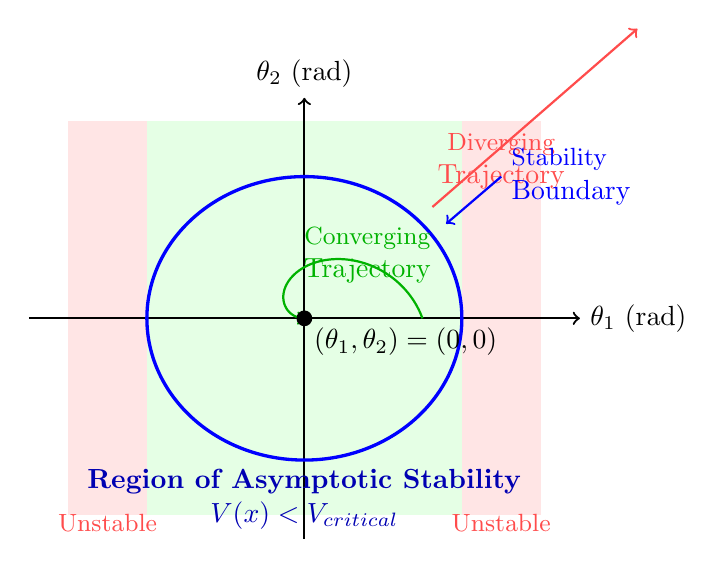
\begin{tikzpicture}[scale=1.0]
    % Background regions
    \fill[green!10] (-3, -2.5) rectangle (3, 2.5);
    \fill[red!10] (-3, -2.5) -- (-2, -2.5) -- (-2, 2.5) -- (-3, 2.5) -- cycle;
    \fill[red!10] (2, -2.5) -- (3, -2.5) -- (3, 2.5) -- (2, 2.5) -- cycle;

    % Axes
    \draw[->, thick] (-3.5, 0) -- (3.5, 0) node[right] {$\theta_1$ (rad)};
    \draw[->, thick] (0, -2.8) -- (0, 2.8) node[above] {$\theta_2$ (rad)};

    % Stability boundary (ellipse for DIP)
    \draw[blue, very thick] (0, 0) ellipse ({2} and {1.8});

    % Sample trajectories
    % Converging trajectory (inside)
    \draw[->, thick, green!70!black, domain=0:180, samples=50, smooth, variable=\t]
        plot ({1.5*cos(\t)*(1-\t/180)}, {1.3*sin(\t)*(1-\t/180)});

    % Diverging trajectory (outside)
    \draw[->, thick, red!70, domain=0:80, samples=30, smooth, variable=\t]
        plot ({2.3*cos(45)*(1+0.02*\t)}, {2.0*sin(45)*(1+0.02*\t)});

    % Equilibrium
    \fill[black] (0, 0) circle (0.1) node[below right] {$(\theta_1, \theta_2) = (0, 0)$};

    % Labels
    \node[green!70!black, align=center] at (0.8, 0.8) {\small Converging\\Trajectory};
    \node[red!70, align=center] at (2.5, 2.0) {\small Diverging\\Trajectory};

    % Region labels
    \node[blue!70!black, align=center] at (0, -2.3) {\textbf{Region of Asymptotic Stability}\\$V(\vect{x}) < V_{\text{critical}}$};
    \node[red!70, align=center] at (2.5, -2.6) {\small Unstable};
    \node[red!70, align=center] at (-2.5, -2.6) {\small Unstable};

    % Boundary annotation
    \draw[<-, thick, blue] (1.8, 1.2) -- (2.5, 1.8) node[right, align=left] {\small Stability\\Boundary};

\end{tikzpicture}
